% !TeX root = ../thuthesis-example.tex

\chapter{斜率优化动态规划}

\section{斜率优化}

斜率优化可以在将转移式变形后,通过考察几何意义,将可能成为最优转移点的集合缩小到一个凸包上,再根据题目条件将转移的时间复杂度缩小到
\(\mathcal{O}(n)\) 或 \(\mathcal{O}(n\log n)\)。

\section{适用问题类型}

可以应用斜率优化的动态规划模型往往某一维度的状态数为 \(\mathcal{O}(n)\)
级别,而为找到最优转移点,单次的状态转移需考察 \(\mathcal{O}(n)\)
个子阶段,这使该维度的转移的时间复杂度开销达到 \(\mathcal{O}(n^2)\)。

\section{应用实例}

\subsection{题目来源}

题目名称:玩具装箱。

题目选自:NOI2008湖南省省队选拔活动。

\subsection{题目描述}

有 \(n\) 个玩具,第 \(i\) 个玩具价值为 \(c_i\)。要求将这 \(n\)
个玩具排成一排,分成若干段。对于一段 \([l,r]\),它的代价为: \[
(r-l+\sum_{i=l}^r c_i-L)^2
\] 求分段的最小代价。

数据范围:\(1\le n\le 5\times 10^4,1\le L,0\le c_i\le 10^7\).

\subsection{解题思路}

令 \(f_i\) 表示前 \(i\) 个物品,分若干段的最小代价。有状态转移方程: \[
f_i=\min_{j<i}{\{f_j+(pre_i-pre_j+i-j-1-L)^2\}}
\] 其中 \(pre_i = \sum_{j=1}^i c_j\)。直接转移时间复杂度为
\(O (n^2)\),无法解决本题。

为简化状态转移方程式,令 \(s_i=pre_i+i,L’=L+1\),则 \[
f_i=\min_{j<i}\{f_j+(s_i-s_j-L’)^2\}
\] 设 \(j\) 为使 \(f_i\) 最小的转移点,有: \[
f_i=f_j+(s_i-s_j-L’)^2
\] 考虑一次函数的斜截式 \(y=kx+b\),将方程转化为这个形式。

其中变量 \(x, y\) 与 \(j\) 有关,\(b, k\) 与 \(i\) 有关,且要求 \(x\) 随
\(j\) 单调递增,仅 \(b\) 中包含 \(f_i\)。

按照上面的规则,对方程进行整理得到: \[
f_j+(s_j+L’)^2=2s_i(s_j+L)+f_i-{s_i}^2
\]

\[
\left\{
\begin{array}{lr}
y = f_j+(s_j+L’)^2\\
k = 2s_i\\
x = s_j+L\\
b = f_i-{s_i}^2
\end{array}
\right.
\]

\((x_j, y_j)\) 的几何意义为直线 \(y=kx+b\)
上的一个点,又因为转移时目的是最小化 \(f_i\),在上面的表示当中,\(f_i\)
只与直线的截距 \(b\) 有关。所以问题可转化为如何选取 \(j\) ,使得过点
\((x_j, y_j)\) 的直线的截距 \(b\) 最小。

注意到直线的斜率不变。如图~\ref{fig:fig1},相当于平移直线 \(y=kx\) ,直到其经过图中的一个点。

\begin{figure}[H]
	\centering
	\begin{framed}
	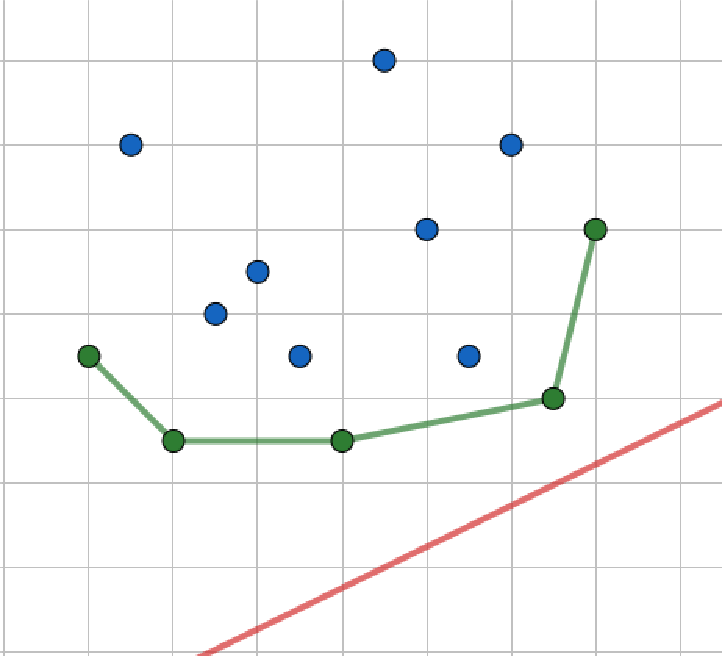
\includegraphics[width=0.5\linewidth]{fig/fig1.pdf}
	\end{framed}
	\caption{}
	\label{fig:fig1}
\end{figure}

% \begin{figure}
%   \centering
%   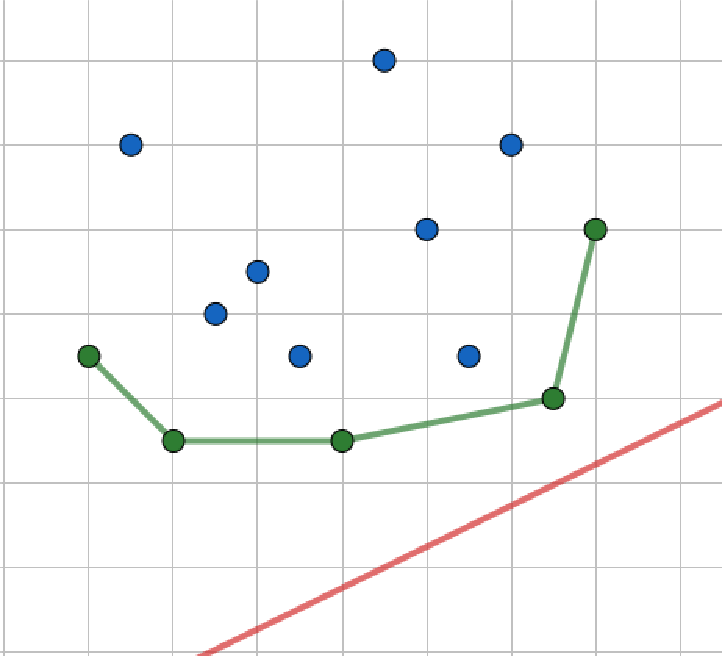
\includegraphics[width=0.6\linewidth]{fig/fig1.pdf}
% %   \caption{图表 1}
%   \label{fig:fig1}
% \end{figure}


于是可以在转移的同时维护 \((x_i,y_i)\)
构成的凸包,利用单调性二分得到时间复杂度为 \(\mathcal{O}(n\log n)\)
的算法。发现 \(k=2s_i\) 关于 \(i\)
单调递增,因此可以利用单调队列来维护得到时间复杂度为 \(\mathcal{O}(n)\)
的算法。

\subsection{代码实现}

6.cpp
